\documentclass[a4paper,11pt]{article}
\usepackage[utf8]{inputenc} %pour utiliser tous les caracteres du clavier 
\usepackage[T1]{fontenc} %meme chose ici
\usepackage[francais]{babel} %pour ecrire en francais
\usepackage{listings} %pour citer du code

\usepackage{amsfonts} % pour utiliser les symboles de ensembles (reel...autre)
\usepackage{amsmath} %debut des package pour utiliser les formules de math
\usepackage{amssymb}
\usepackage{mathrsfs}
\usepackage[top=2cm, bottom=2cm, left=2.0cm, right=1.9cm]{geometry}

\usepackage{graphicx} %pour charger des images
\usepackage{float}

\usepackage{textcomp}
\lstset{
%upquote=true,
columns=flexible,
basicstyle=\ttfamily,}

\title{TP 3 : Application Android: Arboretum\\
Manuel Utilisateur}
\author{Barbier Jérôme, Benyounes Radhoane, Bobo William, Fréby Rodolphe, Husson Augustin, Labat Paul}
\date{\today}

\begin{document}

  \maketitle

  \begin{center}
    
\includegraphics{logoPol.jpg}\\
    %Rapport généré avec \LaTeX
  \end{center}
  \tableofcontents
  \newpage
  
  \section{Introduction}
    Cher lecteur ou lectrice, l'équipe intitulée \textit{Arboricum} est heureuse de vous présenter son application Arboretum qui permet d'avoir une visite 
    guidée du parc du même nom situé sur le campus de Grenoble. \\
    Afin de pouvoir répondre à vos questions et vos attentes, nous mettons à votre disposition ce manuel qui vous guidera sur l'installation de
    notre application dans un premier temps. Ensuite vous aurez tout un descriptif quant à son utilisation.
  \section{Installation}
    \subsection{Configuration}
    Pour faire fonctionner cette application : 
    \begin{itemize}
     \item Vous devez avoir 14,42 Mo de place disponible sur votre espace de stockage interne pour pouvoir installer l'application. Une fois installé, l'application
     aura besoin de 3,5 Mo de plus.
     \item Configuration nécessaire : Android 4.1 avec capteur NFC présent sur votre smarphone/tablette
     \item Vous serez également amenée à autoriser l'application à utiliser : 
     \begin{itemize}
      \item le stockage
      \item votre position (via le GPS)
      \item la communication réseau (c'est à dire avoir un accès Internet complet, ainsi qu'avoir le contrôle NFC
      \item les commandes matérielles (c'est à dire prendre des photos et des vidéos)
     \end{itemize}
    \end{itemize}
NB : tous ces prérequis vous seront donnés avant d'installer l'application.

   \subsection{Installation}
   Il vous suffit de télécharger Arboretum.apk et ensuite de l'installer. Pour le moment l'application n'est pas sûr la plateforme GooglePlay. Donc il 
   vous faudra autoriser votre téléphone a installé des applications non officielle.
   
   Une fois l'application télécharger et installer, il ne vous reste plus qu'à la lancer !!
   
   \section{Utilisation de l'application}
       Lorsque vous utilisez pour la première fois l'application, le fichier grenoble.map va être téléchargé ainsi que Arboretum.map. Il s'agit respectivement de la
       carte de Grenoble et de la carte de l'Arboretum.
    Cette carte est nécessaire pour le fonctionnement de l'application. 3,5 Mo sont nécessaires pour obtenir ces cartes.
    \subsection{Lancement de l'application}
    Une fois l'application lancée, vous arriverez sur le menu de présentation. Vous devrez donc voir apparaître ce que montre les Figures 1 \& 2 (ci-après)
    suivant que vous soyez sur un smarphone ou sur une tablette.
    \begin{figure}[H]
     \begin{center}
      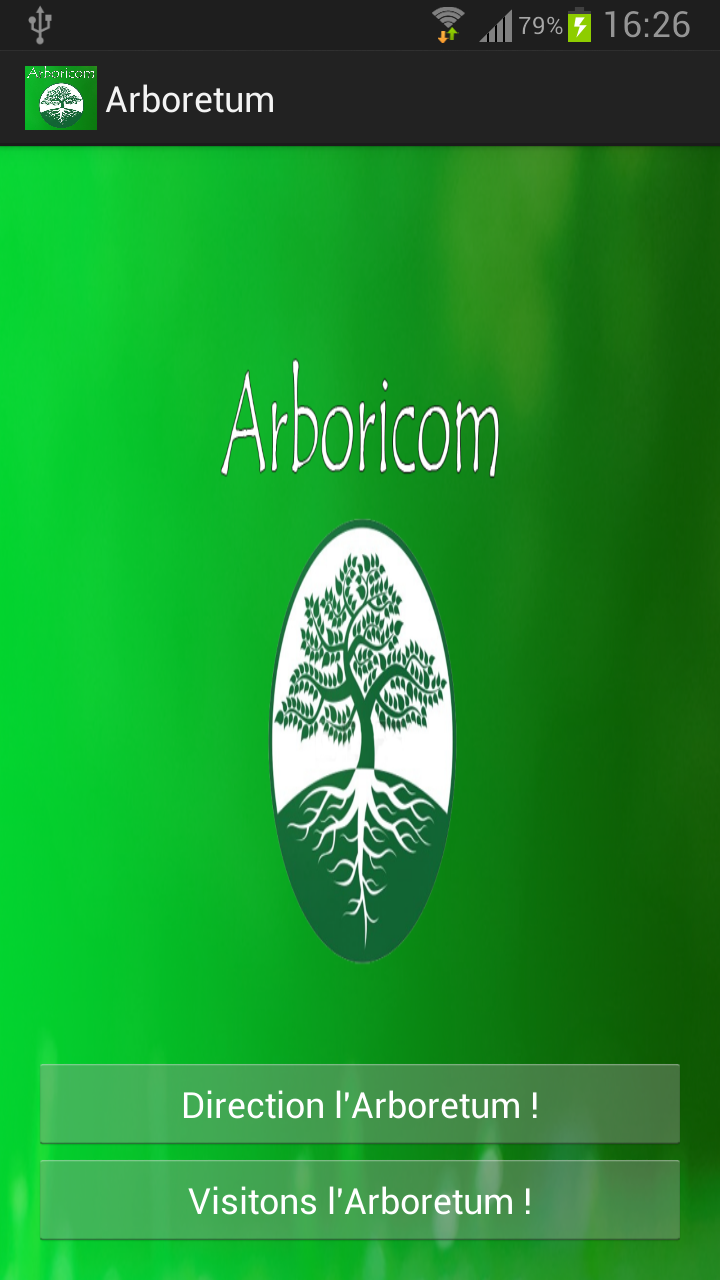
\includegraphics[width=5cm,height=8cm]{menu.png}
      \caption{image du menu de \textit{Arboretum} obtenu sur un \textit{Samsung Galaxy S3}}
     \end{center}
    \end{figure}
    \begin{figure}[H]
     \begin{center}
      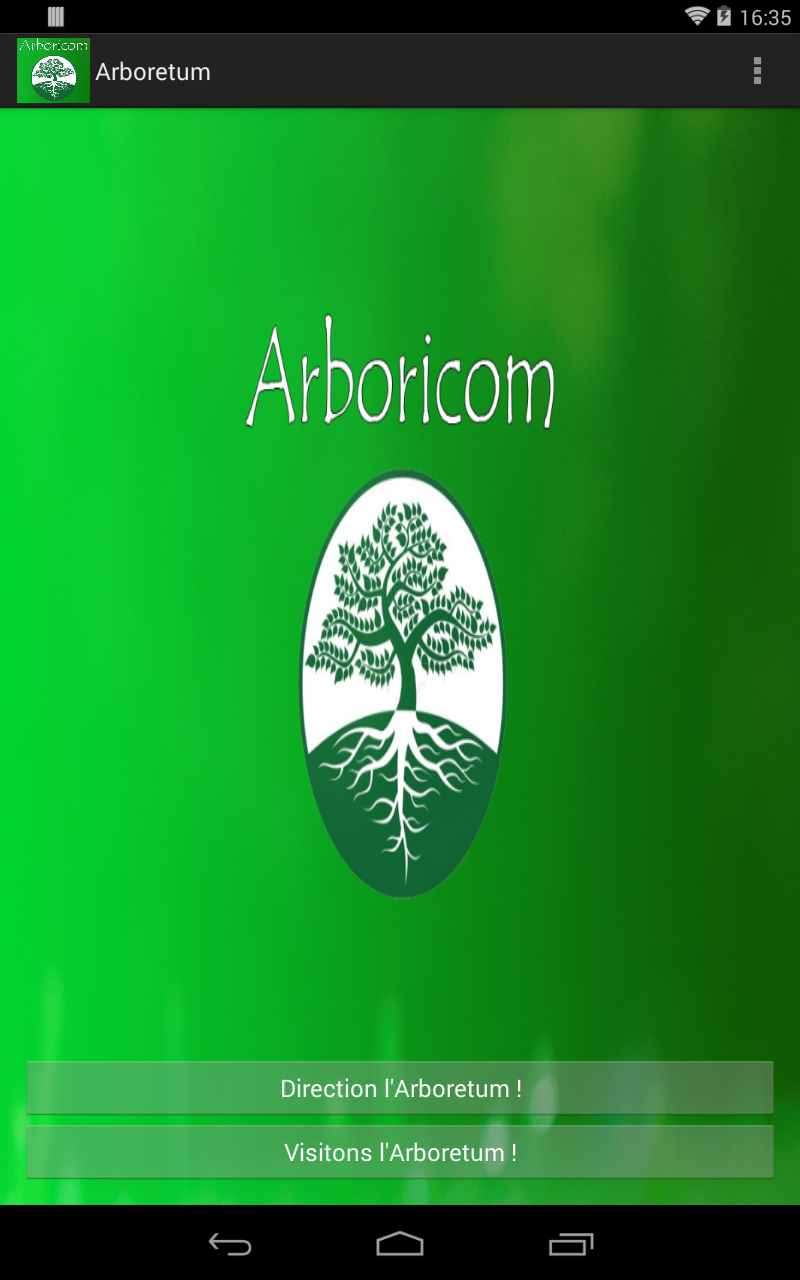
\includegraphics[width=6cm,height=8cm]{menuTablette.png}
      \caption{image du menu de \textit{Arboretum} obtenu sur une tablette \textit{Nexus 7}}
     \end{center}
    \end{figure}
    La différence entre ces deux interfaces se trouve dans le coin en haut à droite. Sur une tablette, vous trouverez 3 petits points. Chose qui
    n'apparaît pas sur un smarphone. Il faudra pour cela appuyer sur le bouton paramètre de votre téléphone.
    
     Si vous êtes sur smarphone, en appuyant sur la touche ``paramètre'', vous obtiendrez 3 nouveaux onglets : 
     \begin{itemize}
      \item Appareil Photo : en cliquant dessus, cela va lancer votre appareil photo 
      \item Son désactivé : il vous suffira de cocher la case associée pour que le son soit désactivé
      \item Crédits : Vous y trouverez les différents membres de l'équipe ainsi que les personnes qui nous ont aidé pour faire ce projet.
     \end{itemize}
         \begin{figure}[H]
     \begin{center}
    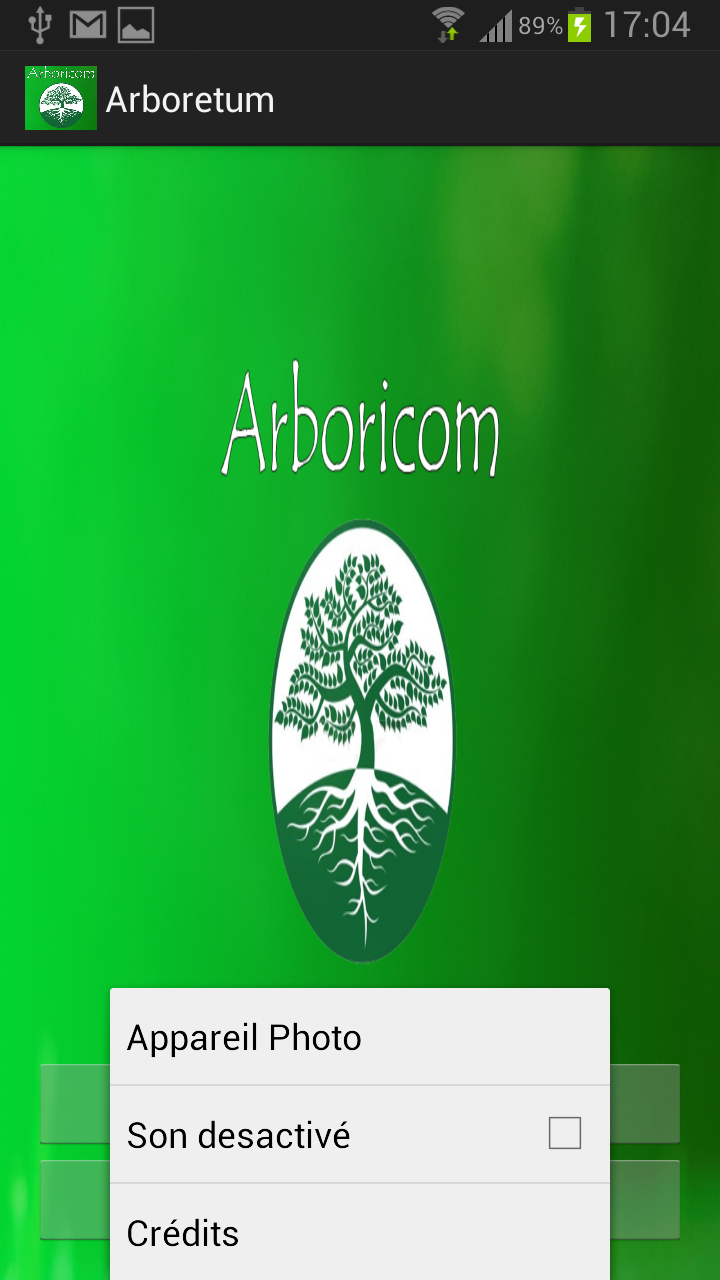
\includegraphics[width=5cm,height=8cm]{menuParamS3.png}
    \caption{image des paramètres de \textit{Arboretum} obtenu sur un \textit{Samsung Galaxy S3}}
     \end{center}
    \end{figure}

    
    Il ne nous reste plus qu'à parler des deux derniers onglets. À savoir : \textit{Direction l'Arboretum} et \textit{Visitons l'Arboretum}
    Le premier onglet vous permettra de rejoindre l'arboretum. Le second vous permettras de le visiter.
    
    \subsection{Direction l'Arboretum}
    Si vous avez cliqué sur le bouton ``Direction l'Arboretum'', c'est donc que vous souhaitez vous y rendre. Il est très probable que vous obteniez
    une page blanche au tout début. Il vous faudra alors dézoomer jusqu'à voir apparaître un ``A'' comme ceci : 
     \begin{figure}[H]
     \begin{center}
      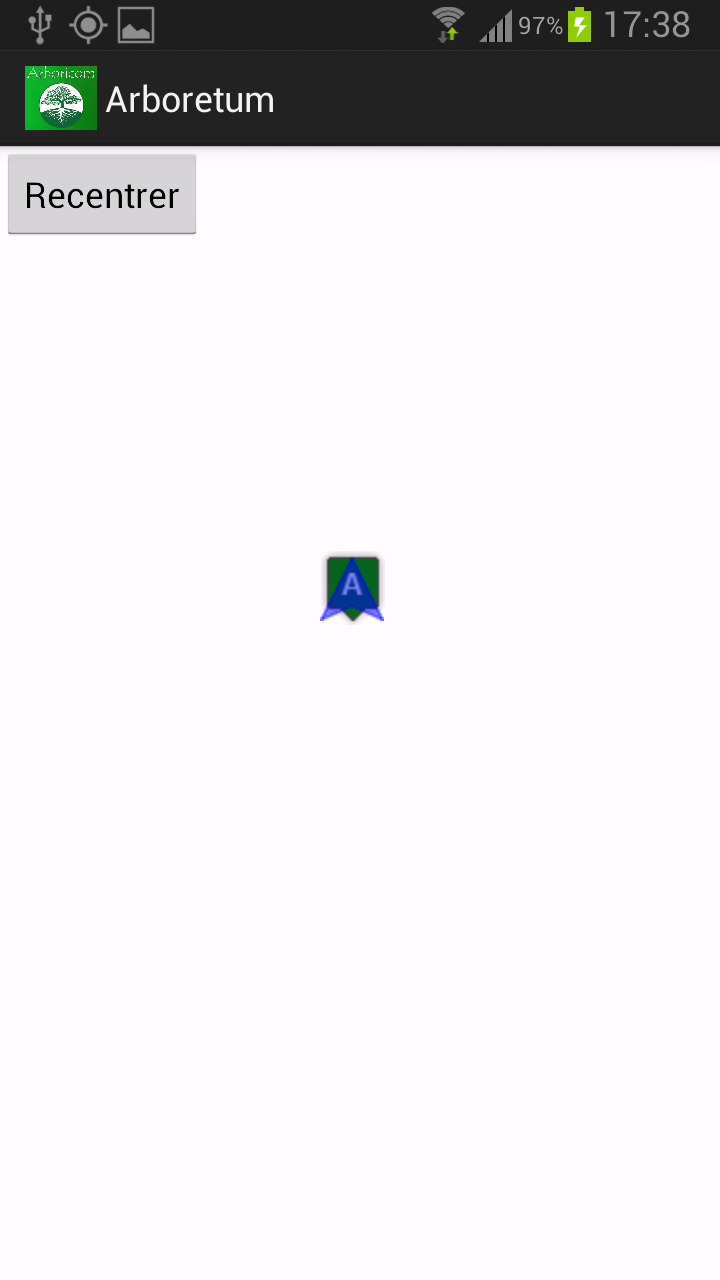
\includegraphics[width=5cm,height=8cm]{pointA.png}
    \caption{Résultat d'un dézoomage}
     \end{center}
    \end{figure}
    \newpage
    Il ne vous restera plus qu'à zoomer sur la position. Vous obtiendrez alors quelques choses de ce genre là :
    \begin{figure}[H]
     \begin{center}
      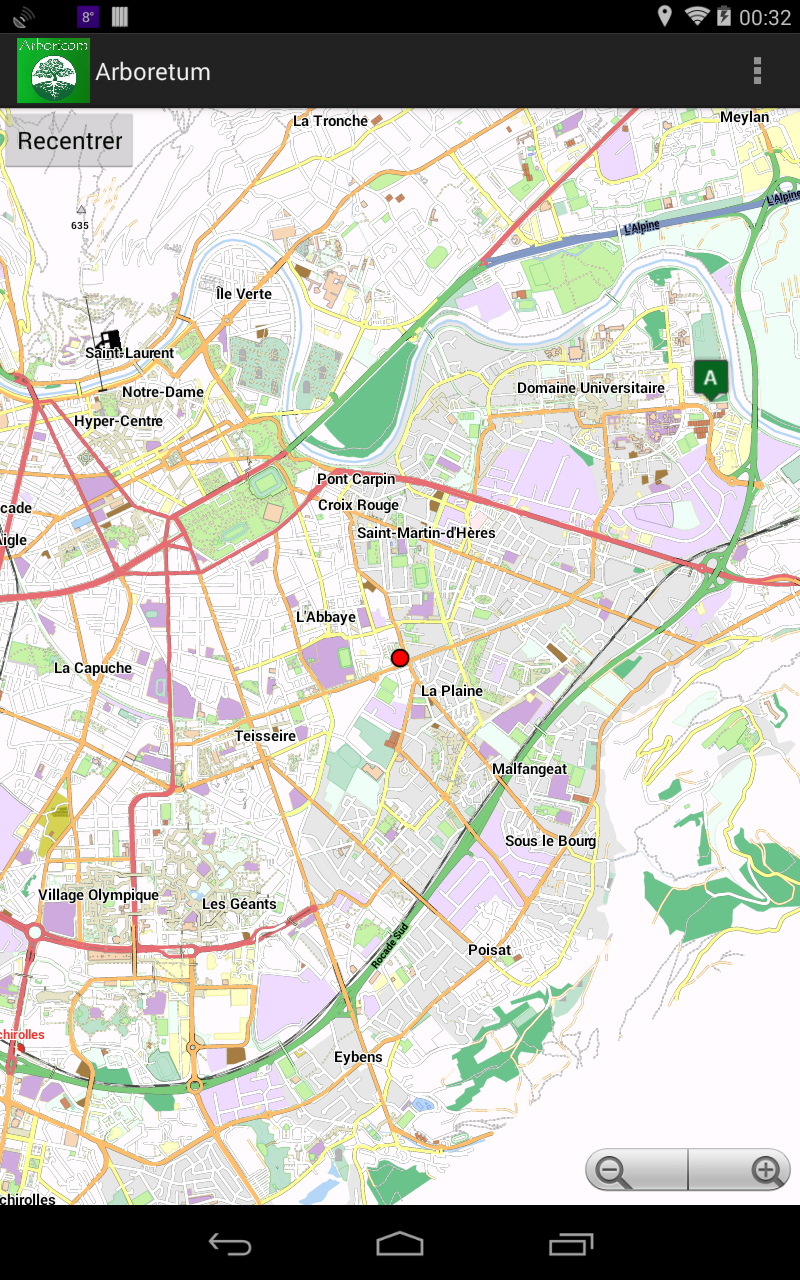
\includegraphics[width=5cm,height=8cm]{grenoble.png}
    \caption{Résultat après un zoomage sur la position}
     \end{center}
    \end{figure}
    
    Comme vous vous en doutez, il s'agit de la carte de Grenoble qui a été télécharger au tout début.
    Vous remarquerez aisément que la flèche bleu indique votre position. Le point ``A'' indique la position de l'arboretum.
    Il ne vous restera plus qu'à trouver un chemin pour vous y rendre.
    
   \textit{NB} : Pour que l'application trouve votre position, vous devez activer le GPS.
   
   \subsection{Visitons L'Arboretum}
    \begin{figure}[H]
     \begin{center}
      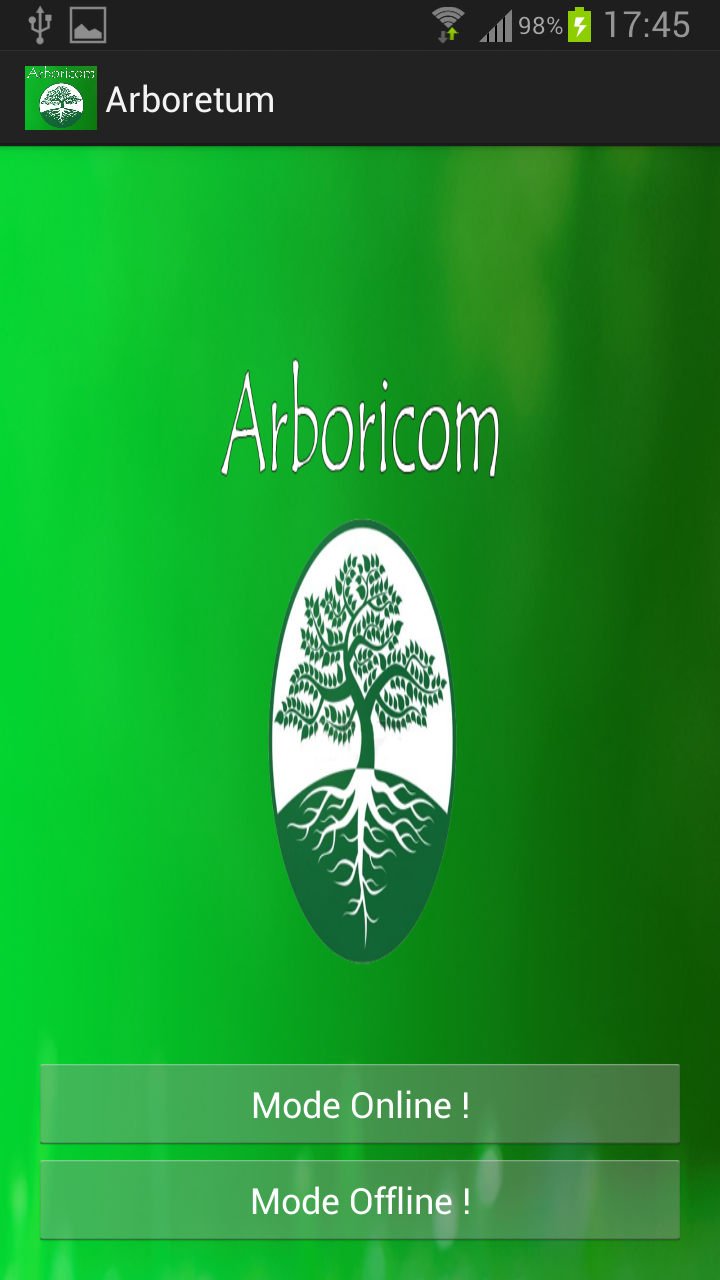
\includegraphics[width=5cm,height=8cm]{visitonsMenu.png}
    \caption{Menu de la fenêtre \textit{Visitons L'Arboretum}}
     \end{center}
    \end{figure}
    \newpage
    Comme vous pouvez le constater, vous vous retrouvez dans un menu et deux choix s'offrent à vous:
    \begin{description}
     \item [Mode Online:] Ce mode est là pour vous faire profiter de la visite du parc en temps réel. Vous devez donc être sur place pour accéder 
     à ce mode.
     \item [Mode Offline:] Ce mode est là pour vous permettre de faire la visite alors que vous n'êtes pas sur place.
    \end{description}
   
   \subsubsection{Le Mode OffLine}
     \begin{figure}[H]
     \begin{center}
      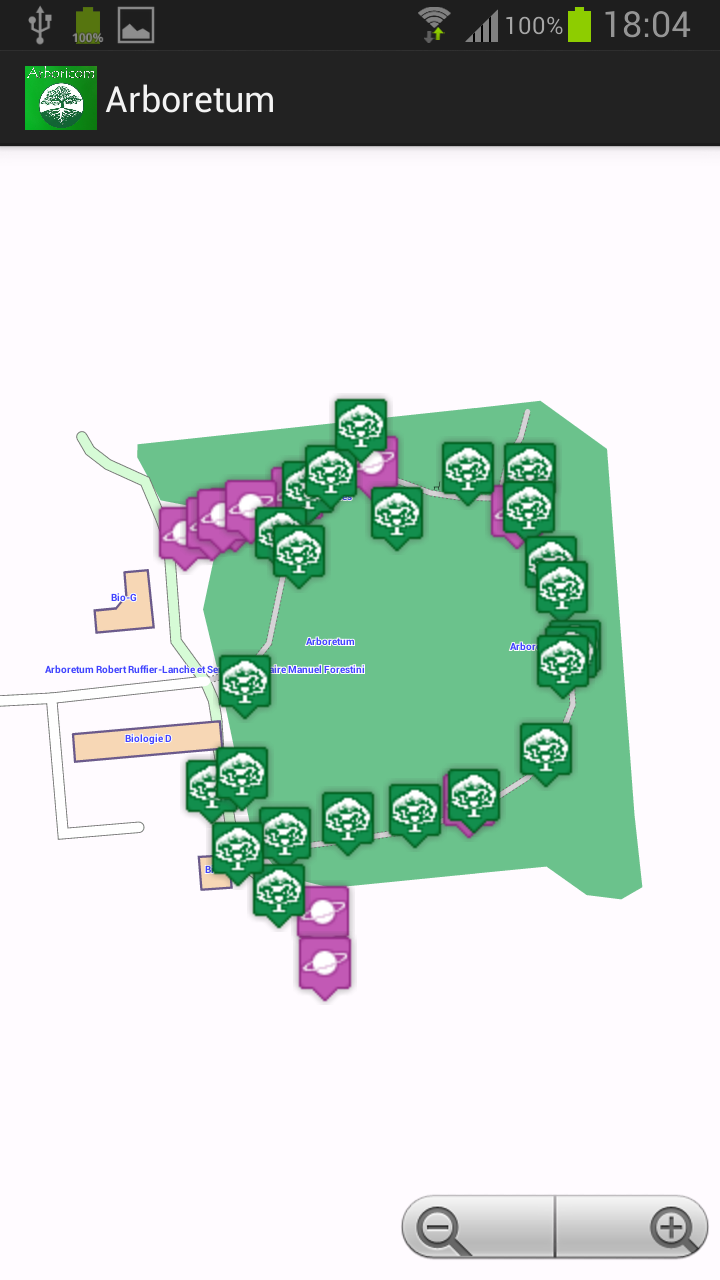
\includegraphics[width=5cm,height=8cm]{modeOffLine.png}
    \caption{Carte de l'arboretum et ses points d'intérêts en mode OffLine}
     \end{center}
    \end{figure}
    
    En cliquant sur le mode Offline, vous voyez alors apparaître la carte du parc. Sur cette carte on retrouvera le sentier qui fait 
    le tour de l'Arboretum, ainsi qu'une multitude de petites images d'arbre et de planètes. 
    
    Vous pouvez bien sûr zoomer sur la carte afin de pouvoir mieux différencier les onglets d'arbre ou de planète.
    Quand vous cliquerez sur arbre vous aurez alors une liste de choix. Il s'agit des variétés végétales que vous auriez trouvé à cet endroit de la carte
    si vous étiez sur place.
    
     \begin{figure}[H]
     \begin{center}
      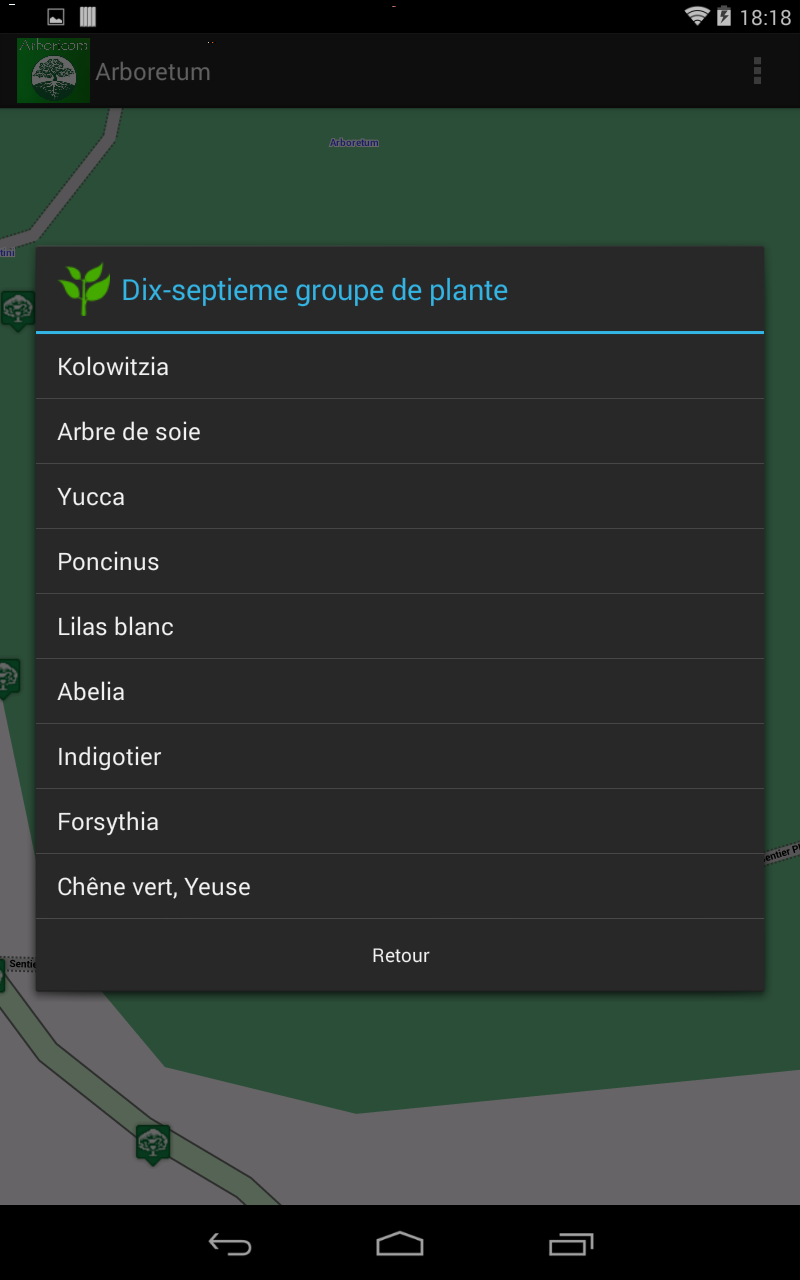
\includegraphics[width=5cm,height=7cm]{choix.png}
    \caption{Liste des plantes après avoir appuyé sur une image de plante}
     \end{center}
    \end{figure}
    
    Après avoir choisis l'un d'entre eux, une page décrivant la plante ou la planète s'ouvrira.
    \begin{figure}[H]
     \begin{center}
      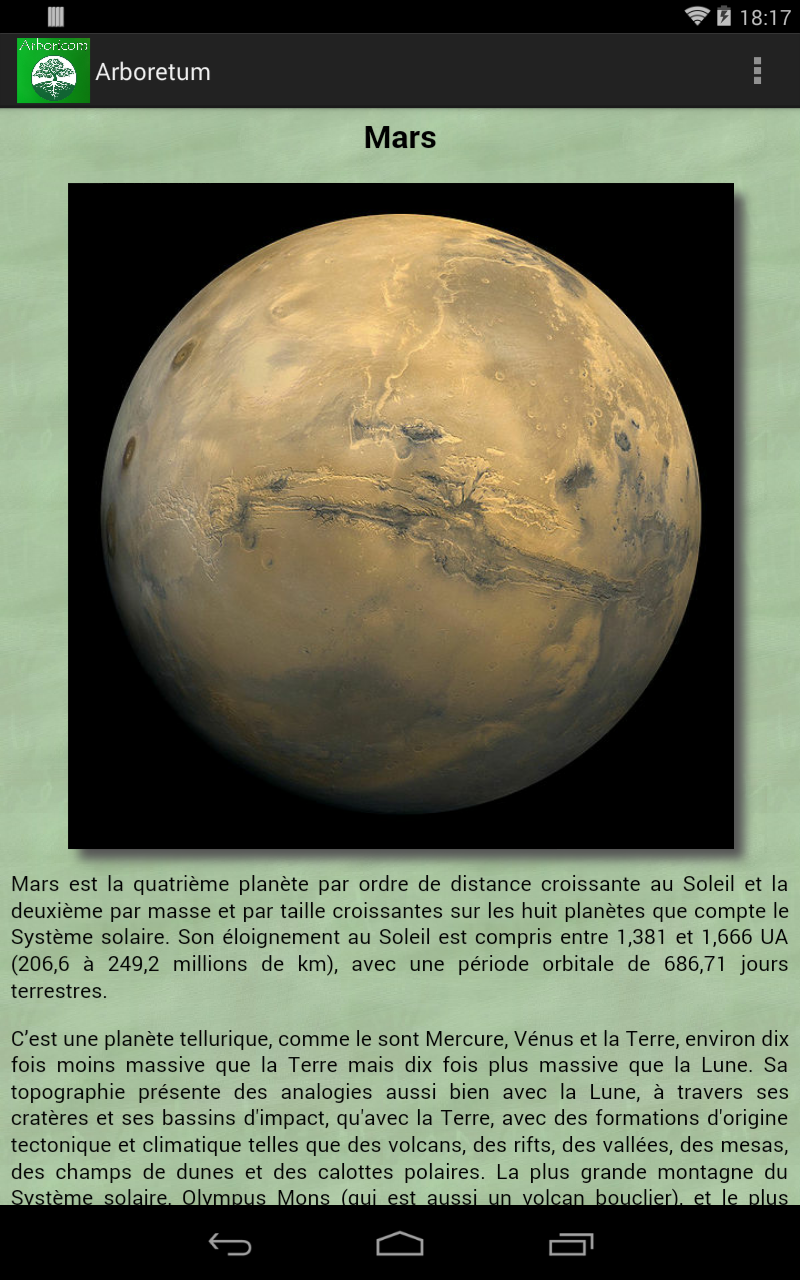
\includegraphics[width=5cm,height=7cm]{mars.png}
    \caption{Description de la planète Mars}
     \end{center}
    \end{figure}
    
    \begin{figure}[H]
     \begin{center}
      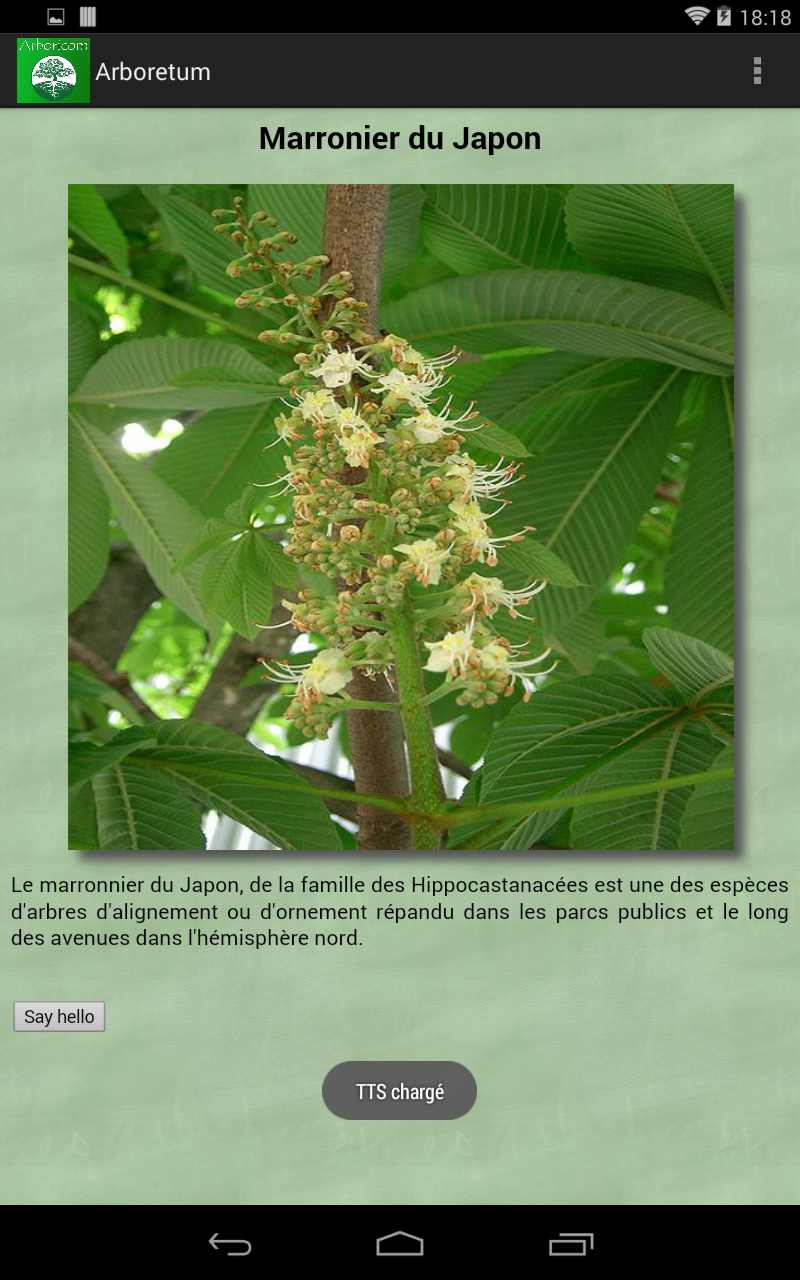
\includegraphics[width=5cm,height=7cm]{marronier.png}
    \caption{Description d'un Marronier du Japon}
     \end{center}
    \end{figure}
    
    \subsubsection*{Le Text To Speach}
    Ou la Synthèse vocale en français, nous avons mis cette fonctionnalité à votre disposition afin que vous puissiez profiter de la visite
    en écoutant simplement les descriptions des différentes plantes et planètes. Pour activer cette fonctionnalité, il suffit d'appuyer sur le bouton
    ``description XXX'' où XXX est le nom de la plante/planète dont vous souhaitez connaître la description.
    
    Une fois après avoir appuyé sur le bouton, vous entendrez une voix qui lira le descriptif écrit sur la page courante.
    
   \subsubsection{Le mode Online}
   Ce mode est très similaire au \textit{Mode Offline} avec les quelques différences que voici : 
   \begin{itemize}
    \item Ce mode nécessite d'avoir activé le GPS 
    \item Suivant votre position, une notification sonore sera faite. Il indiquera que vous vous approchez d'un point d'intérêts (une planète ou une plante)
   \end{itemize}

   \subsubsection*{Utilisation du NFC}
    L'application supporte le NFC. Vous trouverez le long de votre parcours des tags NFC sur les panneaux des planetes et des plantes.
      Si votre appareil est compatible et si vous avez activez le NFC, en posant votre appareil contre le tag, 
      vous aurez des informations supplémentaires sur l'element en face de vous.

   
    \section{Crédits}
    Cette application Android a été réalisé par une équipe d'étudiants en Réseaux Informatiques et Communication Informatique composée par 
    MM. Jérôme BARBIER,Radhoane BENYOUNES, William BOBO, Rodolphe FREBY, Paul LABAT, supervisé par M. Augustin HUSSON et sous la tutelle 
    de M. Jacques LEMORDANT.
    
    \section{Remerciements}
    À Dana Fréby:
    \begin{itemize}
     \item Pour avoir éffectué les relevés GPS nécessaire au positionnement des points d'interêts du parc.
     \item Pour avoir testé le GPS par temps couvert et dégagé. 
     \item Pour avoir testé le son de l'application
    \end{itemize}
    
  À Didier Donzet, pour nous avoir gracieusement donné des tag NFC.

\end{document}
